% Error máximo por lote con aprendizaje iterativo, simulación de lotes de
% 20 kg (An et al., 2018, Tabla 4). Escala: 1 cm por lote, 1,4 cm por kg.
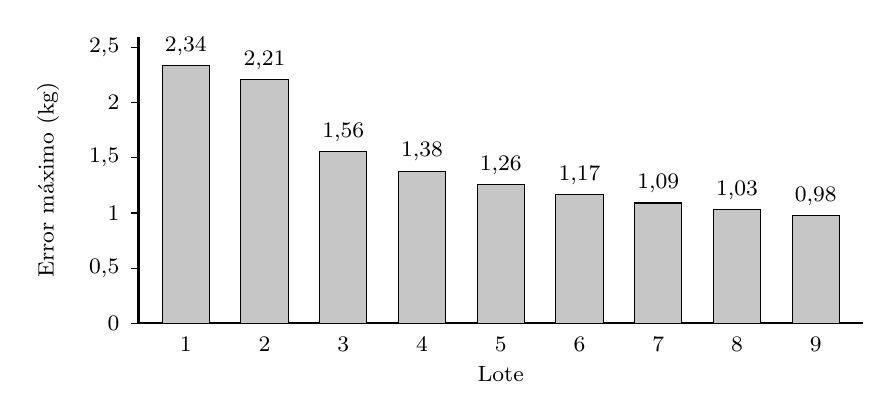
\begin{tikzpicture}[font=\small, nota/.style={font=\footnotesize, align=center}]
\pgfmathsetmacro{\s}{1.4}

% Ejes
\draw[thick] (0.4,0) -- (9.6,0);
\draw[thick] (0.4,0) -- (0.4,{\s*2.6});
\foreach \y in {0,0.5,1.0,1.5,2.0,2.5}{
    \draw (0.4,{\s*\y}) -- (0.3,{\s*\y});
    \node[nota, anchor=east] at (0.28,{\s*\y}) {\pgfmathprintnumber[fixed, precision=1, use comma]{\y}};
}
\node[nota, rotate=90] at (-0.75,{\s*1.3}) {Error máximo (kg)};
\foreach \k in {1,...,9}{\node[nota, anchor=north] at (\k,-0.05) {\k};}
\node[nota] at (5,-0.65) {Lote};

% Barras
\foreach \k/\e in {1/2.34,2/2.21,3/1.56,4/1.38,5/1.26,6/1.17,7/1.09,8/1.03,9/0.98}{
    \fill[gray!45] (\k-0.3,0) rectangle (\k+0.3,{\s*\e});
    \draw (\k-0.3,0) rectangle (\k+0.3,{\s*\e});
    \node[nota, anchor=south] at (\k,{\s*\e}) {\pgfmathprintnumber[fixed, precision=2, use comma]{\e}};
}
\end{tikzpicture}
